\section{HRV appendix}
\subsection{\small ECG signal processing}


\begin{figure}[!htbp]
    \centering
    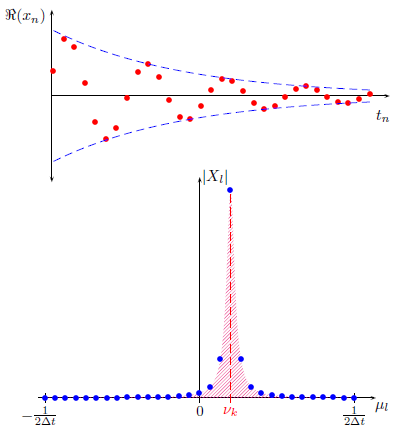
\includegraphics[width=0.5\textwidth]{icon3.png}
    \caption{Electrod placement}
    \label{icon3}
\end{figure}

\begin{figure}[!htbp]
\minipage{0.5\textwidth}%
\centering
    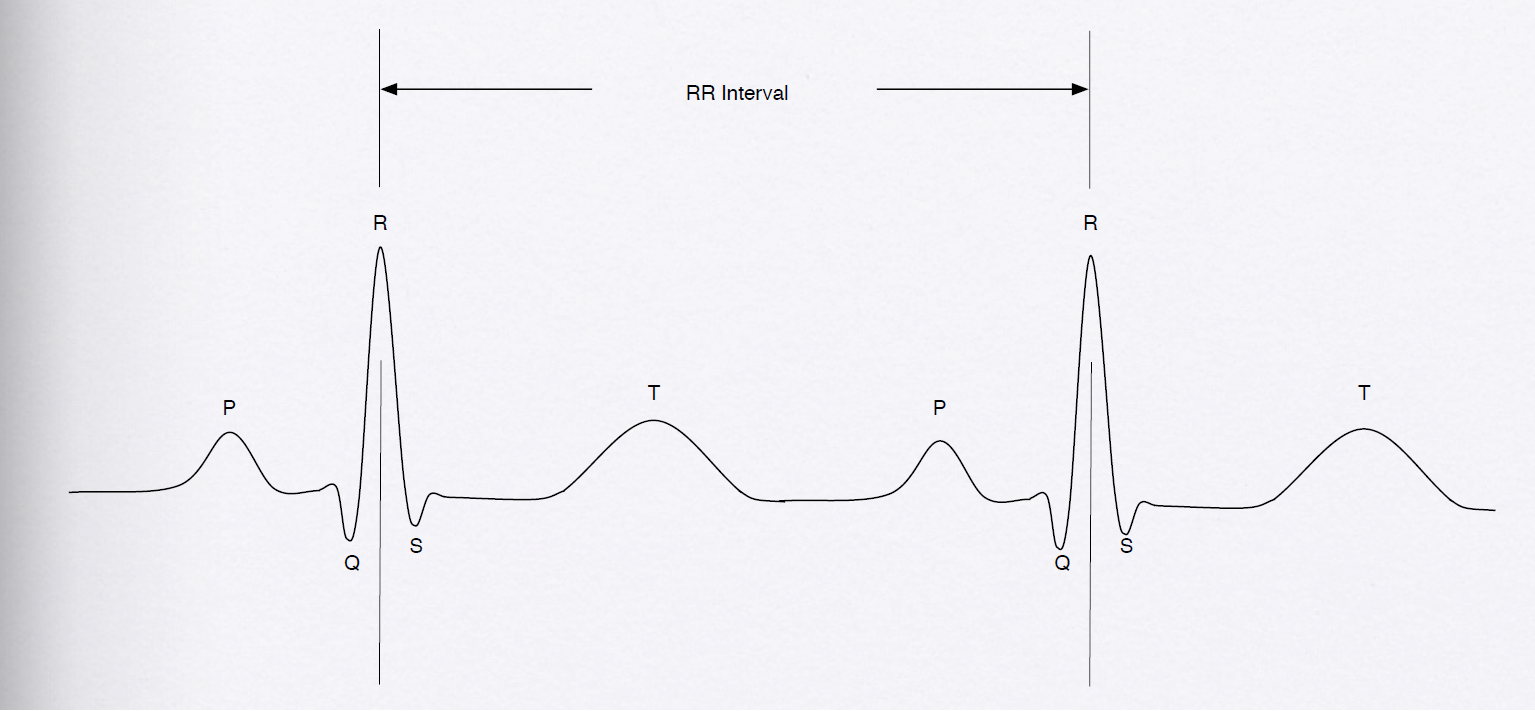
\includegraphics[width=1\textwidth]{icon4.png}
    \subcaption{Outline of heartbeat signal}
\endminipage\hfill
\minipage{0.5\textwidth}%
\centering
    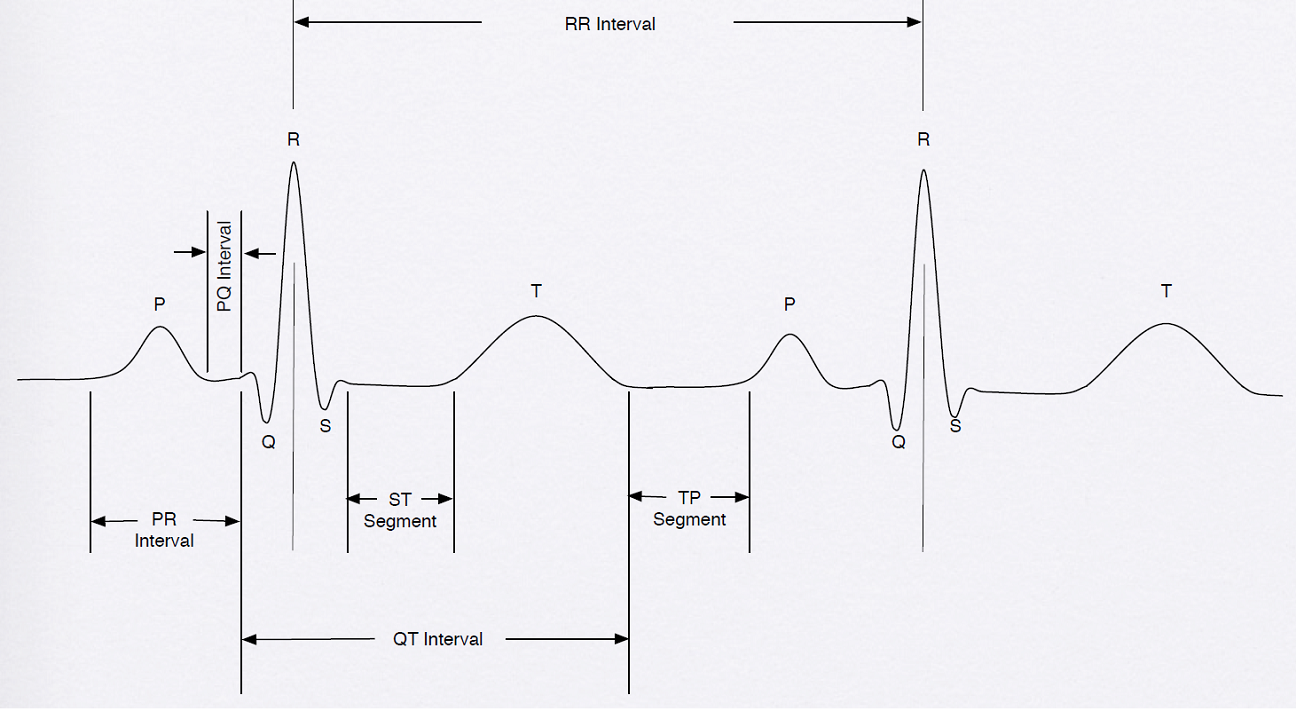
\includegraphics[width=0.9\textwidth]{icon5.png}
    \subcaption{Detailed segmentation of the signal}
\endminipage\hfill
\caption{QRS signal time course}\label{icon4}
\end{figure}

\begin{figure}[!htbp]
\minipage{0.5\textwidth}%
\centering
\begin{itemize}
    \item P wave: depolarisation of atria
    \item QRS complex: depolarisation of ventricles
\end{itemize}
\endminipage\hfill
\minipage{0.5\textwidth}%
\centering
\begin{itemize}
    \item T wave: ventricle re-polarisation
    \item U wave: atria re-polarisation
\end{itemize}
\endminipage\hfill
\caption{QRS signal time course}\label{icon4}
\end{figure}



\newpage
\subsection{\small Pan-Tomkins}\label{algo1}

\begin{figure}[!htbp]
\centering
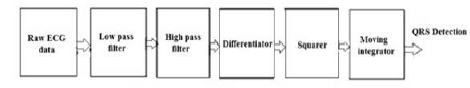
\includegraphics[width=0.6\linewidth]{pan_tomkins.png}
\caption{Pan Tomkins}
\end{figure}


\newpage
\subsection{\small RR time course for each subject of respective group}\label{RR}

\begin{figure}[!htbp]
\foreach \i in {121,...,130} {%
    \begin{subfigure}[p]{0.5\textwidth}
        \includegraphics[width=0.6\linewidth]{\i}
    \end{subfigure}\quad
}
\end{figure}


\newpage
\subsection{\small Pointcare plots}\label{PC}

\begin{figure}[!htbp]
\foreach \i in {131,...,140} {%
    \begin{subfigure}[p]{0.5\textwidth}
        \includegraphics[width=0.6\linewidth]{\i}
    \end{subfigure}\quad
}
\end{figure}

\newpage
\subsection{\small ACF plots}\label{ACF}

\begin{figure}[!htbp]
\foreach \i in {141,...,150} {%
    \begin{subfigure}[p]{0.5\textwidth}
        \includegraphics[width=0.6\linewidth]{\i}
    \end{subfigure}\quad
}
\end{figure}

\newpage
\subsection{\small Phase space plots}\label{PSP}

\begin{figure}[!htbp]
\foreach \i in {151,...,160} {%
    \begin{subfigure}[p]{0.5\textwidth}
        \includegraphics[width=0.6\linewidth]{\i}
    \end{subfigure}\quad
}
\end{figure}

\newpage
\subsection{\small f-slope plots}

\begin{figure}[!htbp]
\foreach \i in {161,...,170} {%
    \begin{subfigure}[p]{0.5\textwidth}
        \includegraphics[width=0.6\linewidth]{\i}
    \end{subfigure}\quad
}
\end{figure}

\newpage
\subsection{\small Hurst exponential plots}

\begin{figure}[!htbp]
\foreach \i in {171,...,180} {%
    \begin{subfigure}[p]{0.5\textwidth}
        \includegraphics[width=0.6\linewidth]{\i}
    \end{subfigure}\quad
}
\end{figure}

\newpage
\subsection{\small Box counting plots}

\begin{figure}[!htbp]
\foreach \i in {181,...,190} {%
    \begin{subfigure}[p]{0.5\textwidth}
        \includegraphics[width=0.6\linewidth]{\i}
    \end{subfigure}\quad
}
\end{figure}




\newpage
\subsection{\small DFA plots}\label{DFAplots}

\begin{figure}[!htbp]
\foreach \i in {191,...,194} {%
    \begin{subfigure}[p]{0.5\textwidth}
        \includegraphics[width=0.6\linewidth]{\i}
    \end{subfigure}\quad
}
\end{figure}

\newpage
\subsection{\small Cumulative plots}\label{CP}

\begin{figure}[!htbp]
\foreach \i in {195,...,204} {%
    \begin{subfigure}[p]{0.5\textwidth}
        \includegraphics[width=0.6\linewidth]{\i}
    \end{subfigure}\quad
}
\end{figure}



\newpage
\subsection{\small Control dataset Correlation dimension plots}

\begin{figure}[!htbp]
\foreach \i in {205,...,214} {%
    \begin{subfigure}[p]{0.5\textwidth}
        \includegraphics[width=0.6\linewidth]{\i}
    \end{subfigure}\quad
}
\end{figure}

\newpage
\subsection{\small Control dataset Correlation dimension plots}
\begin{figure}[!htbp]
\foreach \i in {215,...,224} {%
    \begin{subfigure}[p]{0.5\textwidth}
        \includegraphics[width=0.6\linewidth]{\i}
    \end{subfigure}\quad
}
\end{figure}


\newpage
\subsection{\small Linear regression for window size 16 samples.}\label{LR}

\begin{figure}[!htbp]
\foreach \i in {225,...,234} {
    \begin{subfigure}[p]{0.5\textwidth}
        \includegraphics[width=0.6\linewidth]{\i}
    \end{subfigure}\quad
}
\end{figure}



\end{figure}
